\chapter{Fundamentação teórica e metodologia}\paguso{Chapter title in English}

\paguso{Nesta primeira revisão, eu editei algumas coisas diretamente mas deixei várias outras anotadas pra vc perceber o espírito da coisa. A ideia básica é keep it simple. Quando vc for revisar, releia as frases e veja que palavras são desnecessárias pra compreensão do texto. Se remover uma palavra ou expressão não muda o sentido do texto nem prejudica sua compreensão, não hesite: retire-as. Prefira também orações na voz ativa e na ordem direta sujeito-predicado-complemento.}

\section{\dBG{s}}

% - Detailed explanation of \dBG of a set of DNA sequences
%   - reverse complements
% - How it is going to be used
% - Operations
%   - Insert node
%   - Insert edge
%   - Query node
%   - Query edge / star 
% - Space-efficient representations - that's what we propose

The \keyterm{\dBG of order $k$} of a string \strdef{x}{n}, $G(X;k)=(V,E)$, is defined as the directed graph whose nodes $V$ represent all distinct \kmer{s} of \strname{X}, and such that any two nodes representing $(k-1)$-overlapping \kmers are connected by an edge labeled by the last character of the second \kmer. For example if $k=3$ and $X$ contains the substring \chr{ACGT} then the consecutive triplets \chr{ACG} and \chr{CGT} will originate the edge $\chr{ACG}\stackrel{\chr{C}}{\longrightarrow}\chr{CGT}$. Hence the edges $E$ represent all distinct $(k+1)$-mers of $X$. 
% That is, given two nodes on the graph, they each represent a distinct sequence of symbols $S_1$ and $S_2$, and there is an edge between them if and only if the tail of $S_1$ is the head of $S_2$.
This definition generalizes naturally to a \emph{set of strings} \strsetname{X} by having $G$ to represent all distinct \kmer{s} of all strings in \strsetname{X}.

\change[prefer simple direct forms]{Within the context of}{In} genome sequencing, \dB graphs are used in the assembly process to represent the distinct \kmers in a set \readset of randomly distributed fragments of the source DNA \strname{S}, called \keyterm{reads}, generated by the sequencing machines. \change{In the ideal case}{Ideally}, \strname{S} could be obtained from an Eulerian traversal of $G(\readset, k)$ \cite{}. Unfortunately however, due to sequencing errors and repeats, such a straightforward approach is not feasible, but the \dBG can still be used to produce a collection of partial assemblies, called \keyterm{contigs}, which can then be further combined to form the original genome. Figure~\ref{fig:dbgexample} presents an example of the \dBG \change{within}{in} this context.

\begin{figure}[htbp]
	\begin{center}
    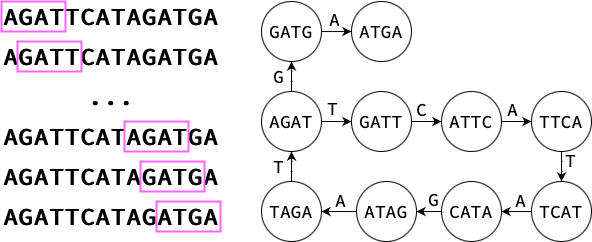
\includegraphics[width=0.8\textwidth]{figures/dbg-example}
	\end{center}
	\caption{Example of a \dBG. $k=4$}\label{fig:dbgexample}
\end{figure}


\subsection{\change{Representing a \dBG}{\dBG representation}}

\asq{Não é mais interessante manter a discussão sobre lower boundaries no capítulo de estado da arte?}

\remove[verbiage]{Due to its nature, a}{A} \dBG can be represented either by its set of nodes (\kmers) or edges ($(k+1)$-mers) equivalently, as one can be derived from the other.
As such, a data structure that can answer queries about the presence of a given node on the graph is enough to
represent the graph. \remove[unnecessary info?]{ Conversely, the same can be achieved with a structure that can answer the same kind of query but about edges. Such structures are called edge-centric, as opposed to the node-centric structures that we consider in this work. Both versions are trivially equivalent, however.} \remove{In this regard, }Conway\&Bromage showed that the lower bound on the space required to
\emph{exactly} represent a \dBG \remove{exists, and} is $\Omega(n \log n)$ bits, \change[always prefer simpler forms]{for $n$ being the number of distinct \kmers present in the graph}{where $n$ is the number of nodes}\remove[isn't this obvious?]{,
and $4^k > n$}\cite{Conway2011}.

In order to further improve space-efficiency, new \remove{forms of} representations were created that trade deterministic exactness for a probabilistic approach. For instance, the so-called \keyterm{Navigational Data Structures} (NDS) have some probability of giving an erroneous answer to a membership query, 
but can still be used to navigate the graph \cite{Chikhi2014}. This \change{definition is useful}{is} due to the fact that a \dBG is usually not queried for membership of \change{randomly selected}{random} nodes, but rather \remove{only} potential neighbors of \change{a known member node is queried}{nodes already known to be in the graph}. In the same paper where they introduce
the idea of NDS \cite{Chikhi2014}\paguso{confirmar referência}, Chikhi \emph{et al.} also present a lower bound for the number of bits needed to represent such a structure as $3.24n$.
In sections \ref{sec:debruijncountmin} and \ref{sec:debruijnhashtable} we will introduce two new NDS's. \asq{É necessário reiterar
os objetivos das duas estrutas aqui, visto que isso já seria feito na introdução e é feito nas próprias sessões dedicadas a cada estrutura?}\paguso{até o momento, acho que não.}

\subsection{Reverse Complements}

\paguso{Esta parte tá meio fora de lugar. Acho que o melhor seria mover a explicação sobre \dBG usando CR para as seção inicial, logo após a figura~\ref{fig:dbgexample}.}
\change{One individuality of the genome sequencing context}{One difficulty of using \dBG{s} to represent DNA data} is the presence of \keyterm{reverse complements}. When generating sequencing reads, \change[prefer active voice]{a sequence of DNA can be read both}{the machine reads either of the two complementary strands of a fragment of the input DNA}. That is, the output read may correspond to the sequence \strname{S} in the forward (5'-3') direction, or its reverse complement \strname{\overline{S}} in the backward (3'-5') direction, with
\strname{\overline{S}} being obtained from \strname{S} by swapping each base with its Watson-Crick complement
($\A \leftrightarrow \T$, $\C \leftrightarrow \G$) and then reversing the string, and vice versa. 
\paguso{Aqui vc já está apresentando sua representação ou discutindo representações em geral? Eu entendo que vc ainda está introduzindo os conceitos.}
As in \cite{Conway2011}, this will be treated by processing
all reads in both directions, without, however, merging nodes representing reverse complements. As noted by Conway \& Bromage: ``This
makes the graph symmetric; a forward traversal corresponds to a backwards traversal on the reverse complement path, and vice versa.``
\cite{Conway2011}


\paguso{Acho que havíamos falado que iríamos introduzir top-down, adiantando o que ia ter na representação, e que operações seriam implementadas, antes de partir para a descrição de cada parte individualmente em detalhes}

\section{The \cm sketch}
\label{sec:countmin}

The \cm sketch \remove{, first introduced in} \cite{Cormode2005} is a \change[acho que quase ninguém usa mais esses hífens]{sub-linear}{sublinear} data structure \remove{intended to allow} for event frequency mapping.
\change{
In this way, it must allow for the query of the frequency of a given event, as well as the update of that frequency, through the
\emph{query} and \emph{update} operations.
}{
It offers two basic operations
\begin{compactenum}
\item $update(e, f)$, and
\item $query(e)$,
\end{compactenum}
respectively for informing the occurrence of an event $e$ with frequency $f$, and for obtaining an estimate of the accumulated frequency of event $e$ up to that point.}

The sketch is composed of a \change{$W$-wide, $D$-deep matrix $C$ of counters.}{$D\times W$ matrix of counters $C$,} \change{With each row in this
matrix is associated a hash function that map the possible events to the $W$ positions in that row.}{and a set of $D$ pairwise-independent hash functions $h_0\ldots h_{D-1}$, such that each $h_i$ maps an event to one of the $W$ cells in row $i$.} \remove{All $D$\/ hash functions
must be pair-wise independent.} 

Updating \change{the frequency of a given}{an} event is done by passing it through the hash functions for each row, and then \change{updating}{incrementing} the counters in
the \change{resulting}{mapped} positions $h_i(e)$ accordingly. 
\change{In this work we take interest in a}{We consider the} simpler case where we only report individual event occurrences, so that counters are always incremented by one.

Querying the structure \change[consists of=to be made up of; consists in=is essentially]{consists of, similarly,}{consists in} retrieving the value of the counters associated with the key event in each row,  and then returning
the minimum value among them, that is $\min\{C[i, h_i(e)]; i=0\ldots D-1$\}.

\asq{É interessante colocar os algoritmos do \cm mais formalmente ou só uma descrição "abstrata" é suficiente?}
\paguso{Acho que assim chega.}


Figure \ref{fig:countminexample} presents a visualization of the \cm sketch.
\paguso{Você ainda não fez o link do uso do CountMin para representar os kmers das sequências, então ainda não é apropriado mostrar um exemplo de CountMin específico para kmers.}

\begin{figure}[htbp]
	\begin{center}
    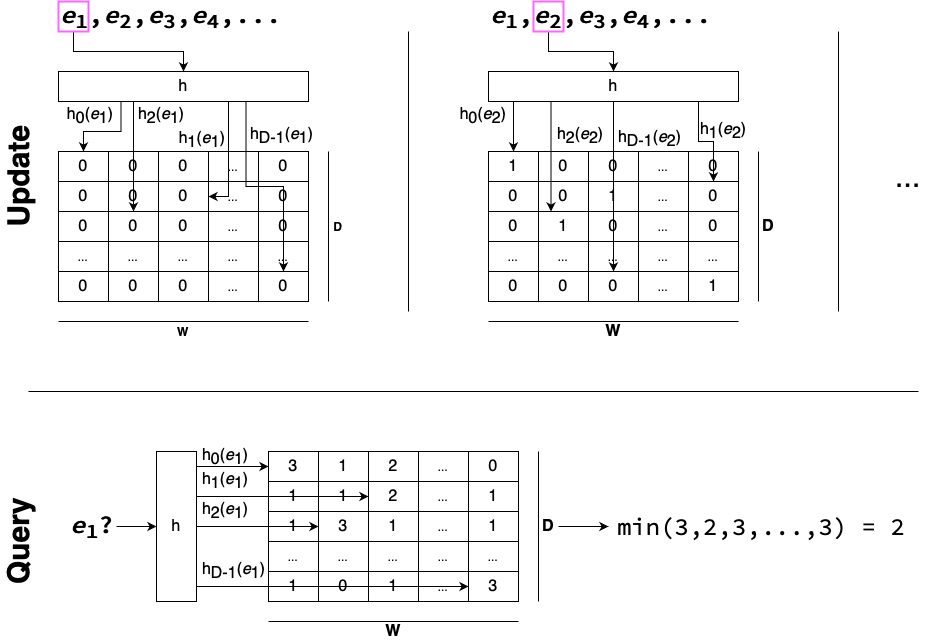
\includegraphics[width=0.8\textwidth]{figures/cm-example}
	\end{center}
	\caption{Example of a \cm sketch being used to count \kmers. $k=4$}\label{fig:countminexample}
\paguso{A ideia da figura está boa, mas precisa aumentar a fonte pra não ficar ilegível. Se não couber, simplifica a parte do incremento. Muda o label de Increment para Update.}
\end{figure}

\paguso{Aqui é importante explicar que o \cm superestima as contagens devido a colisões, mas oferece algumas garantias.}
It is important to notice that the \cm might overestimate the frequency of an event due to hash collisions, since more than one event might be mapped to the same cell of the matrix. However, the pairwise independence requirement ensures that, for any row $i$ and any two distinct events $e\neq e'$,
\begin{equation*}
\prob[h_i(e)=h_i(e')] = 1/W,
\end{equation*}
with this probability being computed over all possible choices of the hash function.
Hence, by setting $W$ appropriately, we can control the expected number of collisions per row, and likewise, by choosing a sufficiently large $D$, we can control for the probability of having at least one row without collisions for a given event. In general, for two given parameters $\epsilon, \delta \in (0,1)$, by setting 
$W=2/\epsilon$ and $D=\log1/\delta$, we have
\begin{equation*}
\prob[C.query(e) - f(e) > \epsilon F] < \delta,
\end{equation*}
where $f(e)$ represents the true frequency of $e$, and $F=\sum_{e_i}f(e_i)$ is the true total event count. Put another way, we can have the estimate error relative to the total event count to be `small' (no more than $\epsilon$) with `good' (at least $1-\delta$) probability.

\subsection{\cm as an intermediate representation for \dBG{s}}

\asq{Vale colocar isso aqui, ou é mais interessante deixar apenas para falar disso no capítulo anterior (State of the Art), quando falando
sobre o \emph{FastEtch}?}
\paguso{Deve migrar essa explicação pro início da Seção \dB \cm}

A \cm sketch can implement the membership query operation by querying the count for a given \kmer and comparing it to a presence threshold:
if the count surpasses this threshold, the \kmer is considered to be present in the \dBG, and if the count is inferior to the threshold the
\kmer is considered absent from the graph.\paguso{Qual é a rationale pra isso? Precisa explicar. Aqui deve ser introduzida a questão da cobertura.} This membership query is defined in Algorithm \ref{alg:countmin-memb}.

\begin{algorithm}[htbp]
  \caption{Membership operation on a \cm sketch}\label{alg:countmin-memb}
  \KwData{$\kmer$; $\mathit{sketch}$, the \cm sketch, $\mathit{threshold}$, the threshold for the presence of a \kmer in the \dBG}
  \Return{$\mathit{sketch}.query(\kmer) \geq \mathit{threshold}$}
  \paguso{Use identificadores mais curtos pras variáveis, tipo $C$: the \cm sketch, $t$: presence threshold. Essas mesmas letras devem ser usadas na explicação no corpo do texto. Este algoritmo em particular pode ser omitido pq é só um teste, e não justifica colocar um Algoritmo separado só pra isso.}
\end{algorithm}

\section{The \dB\cm sketch}
\label{sec:debruijncountmin}

% - Representation (what goes in each cell)
% - Operations:
%   - addOutEdge
%   - query 
% - Analysis space/time (may be done within previous sections)

\asq{Como nós vamos falar das out-edges tanto no \dBCM quanto no \dBHT, poderia ser interessante fazer uma sessão ou subsessão acima
falando sobre o conceito de forma que ele seja apenas referenciado nessas sessões?}


In order to leverage the benefits of using a \cm representation of the \dBG while also improving its navigability, we introduce a modified
version\change{ of the \cm sketch, which we call}{, called} the \keyterm{\dB\cm}, or \dBCM for short, \change{that allows the sketch to be queried}{allowing for querying} not only for \kmer counts, but also for the
\change[sugiro trocar pela versão sem hífen, mais simples e comum]{out-edges}{outedges}  from the \remove{\dBG associated with that \kmer}{corresponding nodes in the graph}. \toconsider{The goal with this modification is to reduce the number of false positives
by querying only the neighbors that are known to possibly exist for that \kmer. This would avoid false paths to be traversed, improving
the trustworthyness of the graph.}\paguso{Sugiro assim: primeiro vc move a explicação de como usar o \cm para \dBG para o início desta Seção (como sugerido acima). Neste ponto, vc pode mencionar que isso permite apenas identificar os nós reais, mas para navegar vc precisa consultar todas as possíveis outeges, o que é lento e abre espaço para FP. Daí vc tem o gancho para introduzir a modificação de guardar essas arestas na própria matriz.}


To store the additional information, we expand the \cm sketch such that each cell $C[i,j]$ in the matrix stores not only the counter,
but also a set of out-edges $C[i,j].E$. The structure then provides an \change{interface}{operation} to \change[que tal manter a interface básica com mesmo nome?]{\emph{increment}}{\emph{update}} the counters associated with a given \change{key}{\kmer} by one,
and an \change{interface}{operation} to \emph{add an out-edge} to the \change[which sets???]{sets}{cells} associated with a given \change{key}{\kmer}. The \change{increment}{update} operation is \change{performed in the same way as in
a regular \cm sketch}{the same as in a regular \cm}, and the \change{algorithm}{procedure} for \change{the add edge operation}{adding an edge} can be seen in Algorithm~\ref{alg:addOutEdge}.


\begin{algorithm}[htbp]
    \caption{Add an out-edge to a \kmer in a \dBCM}\label{alg:addOutEdge}
    \KwData{$\mathit{outEdge} \in \{\A, \C, \G, \T\}$}
    \For{$i = 1, \ldots, D$}{
      $\mathit{CountMin}[i][h_i(\text{k-mer})].\mathit{outEdges} \gets \mathit{CountMin}[i][h_i(\text{k-mer})].\mathit{outEdges} \cup \mathit{outEdge}$\;
    }
\paguso{Eu acho que seria bom tornar as entradas mais explícitas e com nomes mais simples, como as letras usadas na descrição do texto. Algo tipo: \textbf{Input:} $C$ the \dBCM, $x$ the \kmer, $a\in\{\A,\C,\G,\T\}$ the outedge label. Daí a instrução fica algo como $C[i,h_i(x)].E\gets C[i, h_i(x)].E \cup \{a\}$. Fica mais compacto e faz um link com o texto. Algumas coisas nos teus pseudocódigos tão muito ``códigos''.}
\end{algorithm}

Furthermore, the \dBCM must accommodate this new information in its query operation. \change{In order to do this, the}{The} sketch now returns not only
the minimum value of the counters, but also the intersection of the sets of out-edges\change{. The algorithm for the updated query operation is
described}{, as shown in} in Algorithm~\ref{alg:query}.

\begin{algorithm}
	\caption{Query a \kmer in a \dBCM}\label{alg:query}
	$\mathit{count} \gets \mathit{inf}$\;
	$\mathit{outEdges} \gets \{\A, \C, \G, \T\}$\;
	\For{$i = 1, \ldots, D$}{
		$\mathit{count} \gets \min(\mathit{count}, \mathit{CountMin}[i][h_i(\text{k-mer})].\mathit{count})$\;
		$\mathit{outEdges} \gets \mathit{outEdges} \cap \mathit{CountMin}[i][h_i(\text{k-mer})].\mathit{outEdges}$\;
	}
	\Return{$(\mathit{count}, \mathit{outEdges})$}
	\paguso{revisão input e  notação como falei no algoritmo acima}
\end{algorithm}


From a practical perspective, due to a node \change{only ever having 4 possible}{having at most four} out-edges corresponding to the bases $\{\A, \C, \G, \T\}$,
the set storing them can be represented \change{by a bit vector}{with four bits} indicating whether each \change{of these possible edges}{them} is present. An edge is added
by setting the corresponding bit, and the intersection is obtained by performing the bitwise AND operation. \change{This allows both}{Moreover the} set of
out-edges and the counter \change{to be stored}{are packed} together in a single \paguso{16-bit???} integer.\paguso{valia a pena uma figurinha simples aqui com o layout desse inteiro} \toconsider{When using a $k$ such that $4^k > |S|$, the each \kmer in $S$
is expected to appear only once. As such, it is expected to appear a number of times equals to the coverage $C$ in the reads. Considering
that $C$ is not a very high value (commonly below $200$} \asq{Citation Needed?}\toconsider{), each counter can be represented by a 12-bit
integer, accounting for the expected count for all real \kmers, as well as any possible collisions.}\paguso{Sim, acho que deve justificar quantos bits usa e por que.}



\subsection{As a representation of a \dBG}
\paguso{Mudar seção para Using the \dBCM as a navigational structure}

\remove[Essa discussão detalhada do threshold tá redundante.]{As with the \cm sketch, a \dBCM sketch can be queried for membership by comparing the count associated with a given \kmer to a threshold
for presence (i.e. the \kmer is considered present if it appeared $T$ or more times in the reads).} This structure can be navigated from
an initial set of \kmers by querying for their out-edges and then querying each of their neighbors, repeating this when a neighbor is
found to be in the graph. \toconsider{By storing the out-edges, we expect some neighbors to never be explored, reducing the chances of finding
a false path on the graph.}

\paguso{Esta seção deveria focar sobre como pode ser feito um percurso no grafo usando \dBCM. Primeiro vc explica como percorrer a partir de um nó inicial dado. Depois vc explica como candidatos a nós iniciais podem ser obtidos.}

\section{A space-efficiente Hashtable representation for \dBG{s}}
\label{sec:debruijnhashtable}
% - Structure
%   - fingerprint
%   - Outedges
% - Hash function 
% - Collision resolution
% - Operations 
%   - Add node/edge
%   - Query node/edge/star 
% - Analysis 
\paguso{repetindo, é necessário ter discutindo *antes* como essa coisa da hashtable vai colar com o \dBCM, senão isso parece que caiu do céu como uma coisa separada}

We also propose a new hashtable-based representation for the \dBG that is made more efficient by not storing the \kmer. Instead,
a fingerprint generated from the \kmer is stored, along with the set of out edges as described in Section \ref{sec:debruijncountmin}.
When a \kmer is inserted into the hashtable, or queried from it, a hash value and a fingerprint are calculated in parallel.
In case of an insertion, the fingerprint is written at the desired position and, on a query, the fingerprints are compared. Collisions
are resolved by linear probing, such that if a key tries to insert in a position that is already occupied by a fingerprint that doesn't 
match its own, the \kmer is inserted in the next free position, unless its fingerprint is found before a free position is. During the
query this process is repeated until the desired fingerprint is found, or a free position is reached (in which case the \kmer is
considered to be absent from the structure).

This operation allows for the insertion of a node by adding the \kmer to the hashtable, as presented in Algorithm \ref{alg:ht-insert},
and the insertion of an edge by updating the edge set associated with the given \kmer, presented in Algorithm \ref{alg:ht-addedge}.
When queried, the structure returns the edge set associated with the given \kmer, provided the \kmer has been added to the structure.
This operation is defined in Algorithm \ref{alg:ht-query}.

\begin{algorithm}
  \caption{Insert \kmer in \dBHT}\label{alg:ht-insert}
  \KwData{$\kmer$}
  $\mathit{hash} \gets \mathit{fibonacci\_hash}(\kmer)$\;
  $\mathit{pos} \gets \mathit{hash}$\;
  \While{$!\mathit{HT}[\mathit{pos}].empty \wedge \mathit{pos} \neq \mathit{hash} - 1$}{
    \eIf{$\mathit{HT}[\mathit{pos}].\mathit{fingerprint} \neq \mathit{fingerprint}(\kmer)$}{
      $\mathit{pos} \gets (\mathit{pos} + 1) mod |HT|$\;
    }{
      \Return{}
    }
  }
  \If{$\mathit{HT}[\mathit{pos}].empty$}{
    $\mathit{HT}[\mathit{pos}].\mathit{kmer} \gets \kmer$\;
    $\mathit{HT}[\mathit{pos}].\mathit{outEdges} \gets \emptyset$\;
    $\mathit{HT}[\mathit{pos}].\mathit{fingerprint} \gets \mathit{fingerprint}(\kmer)$\;
  }
\end{algorithm}

\begin{algorithm}
  \caption{Add out-edge to \kmer in \dBHT}\label{alg:ht-addedge}
  \KwData{$\kmer$, $\mathit{outEdge} \in \{\A, \C, \G, \T\}$}
  $\mathit{hash} \gets \mathit{fibonacci_hash}(\kmer)$\;
  $\mathit{pos} \gets \mathit{hash}$\;
  \While{$!\mathit{HT}[\mathit{pos}].empty \wedge \mathit{HT}[\mathit{pos}].\mathit{fingerprint} \neq \mathit{fingerprint}(\kmer) \wedge \mathit{pos} \neq \mathit{hash} - 1$}{
    $\mathit{pos} \gets (\mathit{pos} + 1) mod |HT|$\;
  }
  \If{$!\mathit{HT}[\mathit{pos}].empty \wedge \mathit{HT}[\mathit{pos}].\mathit{fingerprint} = \mathit{fingerprint}(\kmer)$}{
    $\mathit{HT}[\mathit{pos}].\mathit{outEdges}.\mathit{add}(\mathit{outEdge})$
  }
\end{algorithm}

\begin{algorithm}
  \caption{Query \kmer in \dBHT}\label{alg:ht-query}
  \KwData{$\kmer$, $\mathit{outEdge} \in \{\A, \C, \G, \T\}$}
  $\mathit{hash} \gets \mathit{fibonacci_hash}(\kmer)$\;
  $\mathit{pos} \gets \mathit{hash}$\;
  \While{$!\mathit{HT}[\mathit{pos}].empty \wedge \mathit{HT}[\mathit{pos}].\mathit{fingerprint} \neq \mathit{fingerprint}(\kmer) \wedge \mathit{pos} \neq \mathit{hash} - 1$}{
    $\mathit{pos} \gets (\mathit{pos} + 1) mod |HT|$\;
  }
  \If{$!\mathit{HT}[\mathit{pos}].empty \wedge \mathit{HT}[\mathit{pos}].\mathit{fingerprint} = \mathit{fingerprint}(\kmer)$}{
    \Return{$\mathit{HT}[\mathit{pos}].outEdges$}
  }
\end{algorithm}

\subsection{Modular Fibonacci Hashing}

The \kmer is hashed using the Fibonacci hashing algorithm, which is an algorithm that leverages a property of the golden ratio
to produce a very uniform hash distribution while also having subsequent keys be hashed to values distant from each other. The
function was modified, however, to use modular arithmetic instead of a bitwise shift operation to map the result to the intended
range. This was done in order to allow for more freedom in the choice of the desired range and, therefore, the size of the
hashtable. The algorithm for this modified version of the Fibonacci hashing function can be seen in Algorithm \ref{alg:fibonacci-hash}.

\begin{algorithm}
  \caption{Fibonacci Hash Function}\label{alg:fibonacci-hash}
  \KwData{$\mathit{key}$; $\mathit{range\_max}$}
  \Return{$(11400714819323198485 \times \mathit{key}) \mod \mathit{range\_max}$}
\end{algorithm}

\subsection{Fingerprint}

When performing the Fibonacci hashing, the most significant bits of the result of the multiplication are discarded by the modulo.
Those bits are also distributed uniformly over the possible keys, such that they can be used as a fingerprint for the \kmer.
As such, the fingerprint function can be defined as in Algorithm \ref{alg:fingerprint}. \asq{Existe uma forma melhor de formalmente
escrever que os $n$ bits mais significativos são escolhidos?}

\begin{algorithm}
  \caption{Fingerprint Function}\label{alg:fingerprint}
  \KwData{$\mathit{key}$}
  \Return{$(11400714819323198485 \times \mathit{key}) >> 61$}
\end{algorithm}

\section{A pipeline using the \dBCM and the \dBHT}

% Sequence ---(insert)---> Mod \cm ---(traverse)---> Hashtable 

Beyond the two isolated datastructures to represent the \dBG, we also propose a way to use both of them in tandem in order to obtain
the benefits of both. In this pipeline, the sequencing reads are processed and inserted into the \dBCM as they are made available,
such that the \dBG can be constructed online. Once the reads are all processed in this manner, and a navigatable version of the graph 
has been constructed, it can be traversed, with all of its nodes being, then, inserted in a \dBHT. In this way, a \dBCM is effectively
compressed into a \dBHT. This pipeline is formalized in Algorithm \ref{alg:pipeline}.

\begin{algorithm}
  \caption{Pipeline using a \dBCM to construct a \dBHT}\label{alg:pipeline}
  \KwData{$R$, a set of sequencing reads}
  $\mathit{dBCM} \gets$ Empty \dBCM sketch\;
  \For{$\mathit{read} \in R$}{
    $\mathit{previous\_\kmer} \gets \emptyset$\;
    \For{$\mathit{kmer} \in \mathit{read}$}{
      $\mathit{dBCM}.\mathit{increment}(\kmer)$\;
      \If{$\mathit{dBCM}.\mathit{query}(\kmer).\mathit{count} \geq T$}{
        $outEdge \gets \kmer[-1]$\;
        $\mathit{dBCM}.\mathit{addOutEdge}(\mathit{previous\_\kmer}, outEdge)$\;
      }
      $\mathit{previous\_\kmer} \gets \kmer$\;
    }
    $\mathit{previous\_\kmer} \gets \emptyset$\;
    \For{$\mathit{kmer} \in \mathit{reverse\_complement(read)}$}{
      $\mathit{dBCM}.\mathit{increment}(\kmer)$\;
      \If{$\mathit{dBCM}.\mathit{query}(\kmer).\mathit{count} \geq T$}{
        $outEdge \gets \kmer[-1]$\;
        $\mathit{dBCM}.\mathit{addOutEdge}(\mathit{previous\_\kmer}, outEdge)$\;
      }
      $\mathit{previous\_\kmer} \gets \kmer$\;
    }
  }
  $\mathit{dBHT} \gets$ Empty \dBHT\;
  \For{$\kmer \in \mathit{dBCM}.\kmers$}{
    $\mathit{dBHT}.\mathit{insert}(\kmer)$\;
    $\mathit{dBHT}[\kmer].\mathit{outEdges} \gets \mathit{dBCM}[\kmer].\mathit{outEdges}$\;
  }
  \Return{$\mathit{dBHT}$}
\end{algorithm}

\section{Experiments}

\subsection{Metrics}

Through the experiments described further in this section, we evaluate different metrics for the \dBCM and the \dBHT. This is due to
the fact that both these structures have different goals and are used in different contexts.

As both of these structures are probabilistic in nature, however, there are certain metrics that are used in the evaluation of both.
One such metric is the \emph{false positive rate}. We define this rate based on the \kmers that are visited during a 
traversal of the graph. Let $S$ be a genetic sequence that contains the set of \kmers $K$, and let $G$ be the graph, represented
either by a \dBCM or a \dBHT, constructed from the sequencing reads of $S$. Further, let $Q$ be the set of \kmers that were queried
from $G$ during its traversal, and $P=\{k | k \in Q \wedge k \in graph\}$ be the set of queried \kmers that were in $G$. As such, we can
define the set of false positives as $F_P=P \setminus K$ (i.e. the set of \kmers that were queried and found to be in $G$ but are not
actually in the original sequence $S$). Finally, the false positive rate is defined as $\mathit{fp}=\frac{|F_P|}{|Q|}$ (i.e. the
proportion of \kmers found during traversal of $G$ that are not found in $K$).

\asq{Realmente vale a pena tentar fazer isso ainda? Estamos na reta final do projeto já, e isso iria requerer a definição do que é uma
mudança significativa nos resultados que justifique a mudança na estrutura}

As we posit that adding the out-edge information to the structures will improve its navigability by reducing the chances of generating
false branches on the graph, we also look at the number of out-edges found for each \kmer in the graph. We can look at the distribution
of these results as a way to evaluate the possible impact of this aditional information: the more \kmers that have fewer out-edges,
the fewer forks there are, and the less likely that a false branch will be generated. \asq{Provavelmente é válido gerar uma formalização
desse conceito de distribuição da contagem de out-edges por \kmer}. Beyond that, we also perform the traversal of the graph with and
without using the out-edge information, such that we can compare the results and measure the impact in this way.

\subsubsection{\dBCM}

The \dBCM was developed to be used directly with the sequencing reads without any pre-processing. It's goal is to build a reliable
navigatable version of the \dBG as the reads are made available. In this context, not only do we expect a certain amount of false
positives will appear, but as we must probabilistically filter the set of \kmers from the reads to remove all the spurious ones, we
also expect the occurence of \emph{false negatives}, which are defined as \kmers from the original sequence $S$ that are not present
in the graph $G$. I.e.: $F_N=K \setminus P$. As such, the \emph{false negative rate} can be defined as the ratio of false negatives
to the total number of \kmers in the original sequence $S$, or $\mathit{fn}=\frac{|F_N|}{|K|}$.

\subsubsection{\dBHT}

\subsection{\emph{E.~Coli}}

The \emph{E.~Coli} genome is an established benchmark for new assemblers to compare against. We used the reference chromossomal dna
genome made available by Ensembl Genomes for the strain k 12, substrain mg1655 of this species\cite{ecoligenome}.

% We used the reference genome for the \emph{E.~Coli} bacterium available in \url{http://ftp.ensemblgenomes.org/pub/bacteria/release-52/fasta/bacteria_0_collection/escherichia_coli_str_k_12_substr_mg1655_gca_000005845/dna/}

Three different experiments were performed. In the first we generated simulated perfect reads from the genome by taking substrings of 
the original sequence at random. We then used the \emph{ART Illumina} toolkit \asq{Citation needed} to simulate realistic reads from this
genome, including read errors and reverse complements. \toconsider{Finally, a dataset of real-world reads was downloaded from SRA \cite{Leinonen2011}
and used.}
\asq{Eu mencionei esse último teste na esperança que dê tempo de realiza-lo ainda.}

\subsubsection{Synthetic reads without errors}

Given the reference genome $S$, the length of each read, $L$, and the desired coverage $C$, the synthetic reads were generated by picking
$\frac{|S| \times C}{L}$ substrings of $S$ at random. This is presented in algorithmic form in Algorithm \ref{alg:generate-reads}.

\begin{algorithm}
  \caption{Generate Reads}\label{alg:generate-reads}
  \KwData{$S$, the reference genome, $L$ the read length, $C$ the coverage}
  $\mathit{\#reads} \gets \frac{|S| \times C}{L}$\;
  $reads \gets \emptyset$\;
  \For{$i \gets 1, \ldots, \mathit{\#reads}$}{
    $j \gets \mathit{random}(0, |S| - L)$\;
    $\mathit{reads.add}(S[j: j+L])$\;
  }
  \Return{$reads$}
\end{algorithm}

\subsubsection{Synthetic reads with errors}

In order to simulate the reads as they would be produced by the sequencing process, we used the ART Illumina toolkit to generate
synthetic reads from the \emph{E.~Coli} genome. The reads were generated using the following parameters:

\begin{enumerate}
\item \textbf{Sequencing System}: Illumina MiSeq v3
\item \textbf{Read length}: \textit{250bp}
\item \textbf{Coverage}: \textit{80x}
\end{enumerate}